% % % % % % % % % % % % % % % % % % % % % % % % % % % % % % % %
% import configuration
% % % % % % % % % % % % % % % % % % % % % % % % % % % % % % % %

% % % % % % % % % % % % % % % % % % % % % % % % % % % % % % % %
% Konfiguration
% % % % % % % % % % % % % % % % % % % % % % % % % % % % % % % %
\newcommand{\titleinfo}{Projektplan}
\newcommand{\subjectinfo}{Widerstands-Berechnungstool}
\newcommand{\authorinfo}{Flurin Arquint, Christoph Hälg, Fabian Söllner, Simeon Roth}
\newcommand{\versioninfo}{1.0}
\newcommand{\docNr}{3.1415}
\newcommand{\dateinfo}{10.10.2019}

% Notes for SRS completion, uncomment the following command to suppress this output
\newcommand{\note}[1]{%
    \vspace{0.25cm}%
    \colorbox{grey}{%
        \parbox{\linewidth-6pt}{%
            \vspace{0.5cm}%
            \centering%
            \parbox{\linewidth-1cm}{%
                \footnotesize{#1}%
            }%
            \vspace{0.5cm}%
        }%
    }%
    \vspace{0.25cm}}
%\newcommand{\note}[1]{}

% % % % % % % % % % % % % % % % % % % % % % % % % % % % % % % %
% Packages, Layout, Units, etc.
% % % % % % % % % % % % % % % % % % % % % % % % % % % % % % % %
%%%%%%%%%%%%%%%%%%%%%%%%%%%%%%%%%%%%%%%%%%
% Dokument
%%%%%%%%%%%%%%%%%%%%%%%%%%%%%%%%%%%%%%%%%%
% Geometrie
\newcommand{\paperFormat}{a4paper}
\newcommand{\lPageMargin}{20mm}
\newcommand{\rPageMargin}{20mm}
\newcommand{\tPageMargin}{20mm}
\newcommand{\bPageMargin}{20mm}

\documentclass[11pt,oneside]{scrartcl}

\newcommand{\newpar}{\par\par}

\usepackage[pdftitle={\titleinfo},%
			pdfauthor={\authorinfo},%
			pdfcreator={pdfLatex, LaTeX with hyperref},
			pdfsubject={\subjectinfo},
			plainpages=false,
			pdfpagelabels,
			colorlinks,
			linkcolor=black,
			filecolor=black,
			citecolor=black,
			urlcolor=black]{hyperref}
						

% Headings
\usepackage{scrlayer-scrpage}


%%%%%%%%%%%%%%%%%%%%%%%%%%%%%%%%%%%%%%%%%%
% Package's
%%%%%%%%%%%%%%%%%%%%%%%%%%%%%%%%%%%%%%%%%%
\usepackage{ucs}
\usepackage[utf8x]{inputenc}
\usepackage[T1]{fontenc}
\usepackage[free-standing-units=true,use-xspace=true]{siunitx}

\usepackage{layout}
\setlength{\parindent}{0em}

\renewcommand{\baselinestretch}{1.2}
\renewcommand{\arraystretch}{1}

%Damit \today ein Deutsch Formatiertes Datum zurueckgibt.
\usepackage[ngerman, num, orig]{isodate}
\usepackage[german, ngerman]{babel}
\monthyearsepgerman{\,}{\,}

\usepackage{amssymb,amsmath,fancybox,graphicx,wrapfig,color,lastpage,verbatim,epstopdf,a4wide,tabularx}
\usepackage{wasysym} %Checkboxen
\usepackage[usenames,dvipsnames]{pstricks}
\usepackage{setspace}
\usepackage{epsfig}
\usepackage{pst-pdf}
\usepackage{pst-all}
\usepackage{pstricks-add}
\usepackage{supertabular}
\usepackage[font=small,labelfont=bf]{caption}
\usepackage[font=footnotesize]{subfig}
\usepackage{footnote}
\usepackage{float}
\usepackage{multirow}
\usepackage{pdfpages}
\usepackage{pgf,tikz}
\usepackage{color}
\usepackage{titletoc}

\usepackage[makeroom]{cancel}
\usepackage{array}
\usepackage{trfsigns}
\usepackage{textcomp}



\renewcommand{\captionfont}{\scriptsize\slshape}
	
\setlength{\unitlength}{1mm}

%Inhaltsverzeichnis
\setcounter{secnumdepth}{4}
\setcounter{tocdepth}{2}

%Geometrie
\usepackage[\paperFormat,left=\lPageMargin,right=\rPageMargin,top=\tPageMargin,bottom=\bPageMargin,includeheadfoot]{geometry}


%%%%%%%%%%%%%%%%%%%%%%%%%%%%%%%%%%%%%%%%%%%%%%%%%%%%%%%%%%%%%%%%
% Environment Numbering
%%%%%%%%%%%%%%%%%%%%%%%%%%%%%%%%%%%%%%%%%%%%%%%%%%%%%%%%%%%%%%%%

%Abbildungsnumerierung anhand Kapitel
\renewcommand{\thefigure}{\arabic{section}.\arabic{figure}}
\makeatletter \@addtoreset{figure}{section} \makeatother

%Gleichungen anhand Kapitel
\AtBeginDocument{\numberwithin{equation}{section}}
\AtBeginDocument{\numberwithin{figure}{section}}
\AtBeginDocument{\numberwithin{table}{section}}


%%%%%%%%%%%%%%%%%%%%%%%%%%%%%%%%%%%%%%%%%%%%%%%%%%%%%%%%%%%%%%%%
% Farben
%%%%%%%%%%%%%%%%%%%%%%%%%%%%%%%%%%%%%%%%%%%%%%%%%%%%%%%%%%%%%%%%
\definecolor{black}{rgb}{0,0,0}
\definecolor{red}{rgb}{1,0,0}
\definecolor{white}{rgb}{1,1,1}
\definecolor{grey}{rgb}{0.8,0.8,0.8}


%%%%%%%%%%%%%%%%%%%%%%%%%%%%%%%%%%%%%%%%%%%%%%%%%%%%%%%%%%%%%%%%
% Einheiten
%%%%%%%%%%%%%%%%%%%%%%%%%%%%%%%%%%%%%%%%%%%%%%%%%%%%%%%%%%%%%%%%
%\usepackage[Gray,squaren]{SIunits} %\gray befehl heisst nun \Gray und \square heisst nun \squaren
% replaced by \usepackage[free-standing-units=true,use-xspace=true]{siunitx} but at the beginning of the document

%Spannung
\DeclareMathOperator{\V}{\volt}
\DeclareMathOperator{\mV}{\milli \volt}
\DeclareMathOperator{\uV}{\micro \volt}

%Strom
\DeclareMathOperator{\A}{\ampere}
\DeclareMathOperator{\mA}{\milli \ampere}
\DeclareMathOperator{\uA}{\micro \ampere}
\DeclareMathOperator{\nA}{\nano \ampere}

%Zeit
\DeclareMathOperator{\s}{\second}
\DeclareMathOperator{\ms}{\milli \second}
\DeclareMathOperator{\us}{\micro \second}
\DeclareMathOperator{\ns}{\nano \second}

%Kapazitaet
\DeclareMathOperator{\mF}{\milli \farad}
\DeclareMathOperator{\uF}{\micro \farad}
\DeclareMathOperator{\nF}{\nano \farad}
\DeclareMathOperator{\pF}{\pico \farad}
\DeclareMathOperator{\fF}{\femto \farad}

%Induktivitaet
\DeclareMathOperator{\mH}{\milli \henry}
\DeclareMathOperator{\uH}{\micro \henry}
\DeclareMathOperator{\nH}{\nano \henry}

%Widerstand
\DeclareMathOperator{\MO}{\mega \ohm}
\DeclareMathOperator{\kO}{\kilo \ohm}
\DeclareMathOperator{\mO}{\milli \ohm}
\DeclareMathOperator{\Ohm}{\ohm}
%Strecke
\DeclareMathOperator{\km}{\kilo \meter}
\DeclareMathOperator{\cm}{\centi \meter}
\DeclareMathOperator{\mm}{\milli \meter}

%Frequenz
\DeclareMathOperator{\GHz}{\giga \hertz}
\DeclareMathOperator{\MHz}{\mega \hertz}
\DeclareMathOperator{\Hz}{\hertz}
\DeclareMathOperator{\kHz}{\kilo \hertz}
\DeclareMathOperator{\mHz}{\milli \hertz}

%Leistung
\DeclareMathOperator{\kW}{\kilo \watt}
\DeclareMathOperator{\mW}{\milli \watt}
\DeclareMathOperator{\uW}{\micro \watt}
\DeclareMathOperator{\W}{\watt}

%Kreisfrequenz
\DeclareMathOperator{\rpers}{\radianpersecond}

%DeziBel
\DeclareMathOperator{\dB}{\deci \bel}
\DeclareMathOperator{\dBm}{\deci \bel \milli}

%Bit
\DeclareMathOperator{\Bit}{\text{Bit}}
\DeclareMathOperator{\kBit}{\text{kBit}}
\DeclareMathOperator{\MBit}{\text{MBit}}
\DeclareMathOperator{\Byte}{\text{Byte}}
\DeclareMathOperator{\kByte}{\text{kByte}}
\DeclareMathOperator{\MByte}{\text{MByte}}
\DeclareMathOperator{\ppm}{\text{ppm}}

% % % % % % % % % % % % % % % % % % % % % % % % % % % % % % % %
% Dokument
% % % % % % % % % % % % % % % % % % % % % % % % % % % % % % % %
\begin{document}

% % % % % % % % % % % % % % % % % % % % % % % % % % % % % % % %
% Titelseite
% % % % % % % % % % % % % % % % % % % % % % % % % % % % % % % %
\newgeometry{left=20mm, right=20mm, top=10mm, bottom=10mm}

\hrule
\begin{tikzpicture}[scale=1]
\node[] at(0cm,0) {
\includegraphics[height=1.5cm,trim=0mm 2mm 0cm 0mm, clip]{content/title/HSR_Logo_CMYK.eps}};			
\end{tikzpicture}
\hrule
\begin{center}
   	\vspace*{\stretch{1}}
   	\begin{flushright}
   		\Huge
   		\titleinfo\\
   		\Large
   		Projekt: \subjectinfo\\
   		\large
   		\vspace*{\stretch{0.1}}
   		Version \versioninfo\\
   		\vspace*{\stretch{0.5}}
   		\authorinfo \\			
   	\end{flushright}
   	\vspace*{\stretch{2}}	
   	\newcolumntype{Y}{>{\setlength\hsize{0.4\hsize}\raggedright\arraybackslash}X}
   	\newcolumntype{Z}{>{\setlength\hsize{0.3\hsize}\raggedright\arraybackslash}X}
   	\renewcommand\arraystretch{1.5}
   	\begin{tabularx}{\linewidth}{|Z|Y|Z|}
   		\hline
   		\textbf{Name} & \textbf{Datum} & \textbf{Unterschrift}\\
   		\hline
   		Flurin Arquint & \printdate{\dateinfo} & \\
   		\hline
   		Christoph Hälg & \printdate{\dateinfo} & \\
   		\hline
   		Fabian Söllner & \printdate{\dateinfo} & \\
   		\hline
   		Simeon Roth & \printdate{\dateinfo} & \\
        \hline
   	\end{tabularx}
\end{center}
\cfoot{}
\vspace*{\stretch{0.5}}	
\hrule
{
    \footnotesize 
    \begin{flushright}
        Doc\#: \docNr\linebreak
        Datum: \dateinfo
    \end{flushright}
}

\restoregeometry
	
% % % % % % % % % % % % % % % % % % % % % % % % % % % % % % % %
% Kopf und Fuszeile aktivieren

\pagestyle{scrheadings}
\KOMAoption{headsepline}{true}
\KOMAoption{footsepline}{true}
\ihead{\footnotesize\normalfont \titleinfo}
\ohead{\footnotesize\normalfont \subjectinfo}
\cfoot{}
\setkomafont{pagenumber}{\normalfont}
\ofoot{\footnotesize\normalfont\pagemark\ von \pageref{LastPage}}
\ifoot{\footnotesize\normalfont\copyright\ HSR Hochschule für Technik Rapperswil 2019}


% % % % % % % % % % % % % % % % % % % % % % % % % % % % % % % %
% Revision History
% % % % % % % % % % % % % % % % % % % % % % % % % % % % % % % %	
\section*{Änderungsübersicht}
\begin{tabular}{lcll}
    \textbf{Datum} & \textbf{Version} & \textbf{Autor} & \textbf{Beschreibung}\\
    2019-10-10 & 0.1 & F.Arquint, C.Hälg, F.Söllner, S.Roth& Projektplan erstellt \\
\end{tabular}

%\note{
%    Die Information in dieser Tabelle muss nur dann aktualisiert werden,
%    wenn eine neue Version des Dokumentes erzeugt, bzw. freigegeben wird,
%    nicht aber jedes Mal wenn das Dokument 'angefasst' wird.
%}

\contentsfinish
% % % % % % % % % % % % % % % % % % % % % % % % % % % % % % % %
% General notes
% % % % % % % % % % % % % % % % % % % % % % % % % % % % % % % %	
\note{
\begin{itemize}
%\item Alle Abschnitte, die im Style "Comment" geschrieben sind (wie dieser Text), dienen nur für Erklärungen, die dem Autoren des Dokumentes helfen sollen. Diese Kommentare müssen im endgültigen Dokument entfernt oder unsichtbar gemacht werden.
%
%\item Im Dokument werden verschiedene Felder, z.B. für das Datum, den Projektnamen, etc. verwendet. Diese sollen deshalb unbedingt zu Beginn unter den Doc properties (Dokumenteigenschaften) festgelegt werden.
%
\item Die hier präsentierte Pflichtenheftvorlage ist angelehnt an \textbf{IEEE Recommended Practice for Software Requirements Specification. ANSI/IEEE Std 830-1998}. Sie kann auch für Projekte verwendet werden, die nicht nur aus Software bestehen.
%
\item Gemäss DIN 69901-5 umfasst das Pflichtenheft die "vom Auftragnehmer erarbeiteten Realisierungsvorgaben aufgrund der Umsetzung des vom Auftraggeber vorgegebenen Lastenhefts", d.h. das Lastenheft beinhaltet die Kundenanforderungen, im Pflichtenheft sind technische Vorgaben an die Entwicklungsgruppe formuliert, z.B. allenfalls notwendige Vorgaben für die Programmiersprache, die Plattformen, Betriebssystem, etc... Im Pflichtenheft darf keinesfalls das Design beschrieben werden.
%
\item Im internationalen Umfeld werden statt der DIN-Normen eher die IEEE-Normen angewandt. Im IEEE Standard 830 wird eine "Software Requirements Specification" formuliert, welche sowohl das Lastenheft als auch das Pflichtenheft beinhaltet. Diese Vorlage verfolgt diesen Ansatz. Teilweise werden Hinweise in Englisch direkt aus diesem Standard verwendet. Weitere Informationen zu den einzelnen Punkten finden Sie direkt in \cite{ieeeStd}.
%
\item The Requirements Specification should address the product, not the process of producing the product. Project requirements represent an understanding between the customer and the supplier about contractual matters pertaining to production of the product and thus should not be included in the Requirements Specification. These normally include items such as
	\begin{itemize}
	\item Cost
	\item Delivery schedules
	\item Reporting procedures
	\item Development methods
	\item Quality assurance
	\item Validation and verification criteria
	\item Acceptance procedures
	\end{itemize}
Project requirements are specified in other documents, typically in a software development plan, a software quality assurance plan, or a statement of work.
\end{itemize}
\clearpage
}

\newpage
	
% % % % % % % % % % % % % % % % % % % % % % % % % % % % % % % %
% Inhaltsverzeichnis
% % % % % % % % % % % % % % % % % % % % % % % % % % % % % % % %

	{\linespread{1.0} \tableofcontents}
	\newpage
	
		
% % % % % % % % % % % % % % % % % % % % % % % % % % % % % % % %
% Kapitel
% % % % % % % % % % % % % % % % % % % % % % % % % % % % % % % %
	\newpage
		
	%damit " kein umlaut erzeugt und als Anführungszeichn verwendet werden kann
	\shorthandoff{"} %Abschalten mit\shorthandon{"}
    
    % Abbildungen
    \listoffigures
    \addcontentsline{toc}{subsection}{Abbildungsverzeichnis}
        
    % Tabellen
    \listoftables
    \addcontentsline{toc}{subsection}{Tabellenverzeichnis}
			
	%Includes	
	\section{Einleitung}
\label{sec:intro}

\subsection{Zweck}
Im vorliegenden Dokument sind die Anforderungen definiert, welche im Projekt \subjectinfo\ umgesetzt werden müssen. 
Es beschreibt den Auftrag zwischen Auftraggeber und Auftragnehmer. 
Der Ausdruck Pflichtenheft ist hier im Sinne der IEEE Recommended Practice for Software Requirements Specification. ANSI/IEEE Std 830-1998 verwendet.
Die dort definierte Requirements Specification beinhaltet sowohl die Benutzeranforderungen (Lastenheft gemäss DIN 69901-5) als auch Realisierungsvorgaben an die Entwicklungsgruppe (Pflichtenheft gemäss DIN 69901-5).

\subsection{Produktüberblick}
Im Rahmen dieses Projekt soll eine Software entwickelt werden, welche das optimale Spannungsteiler Widerstandsverhältnis für einen unbelasteten Spannungsteiler berechnet.
\begin{figure}[!h]
	\centering
	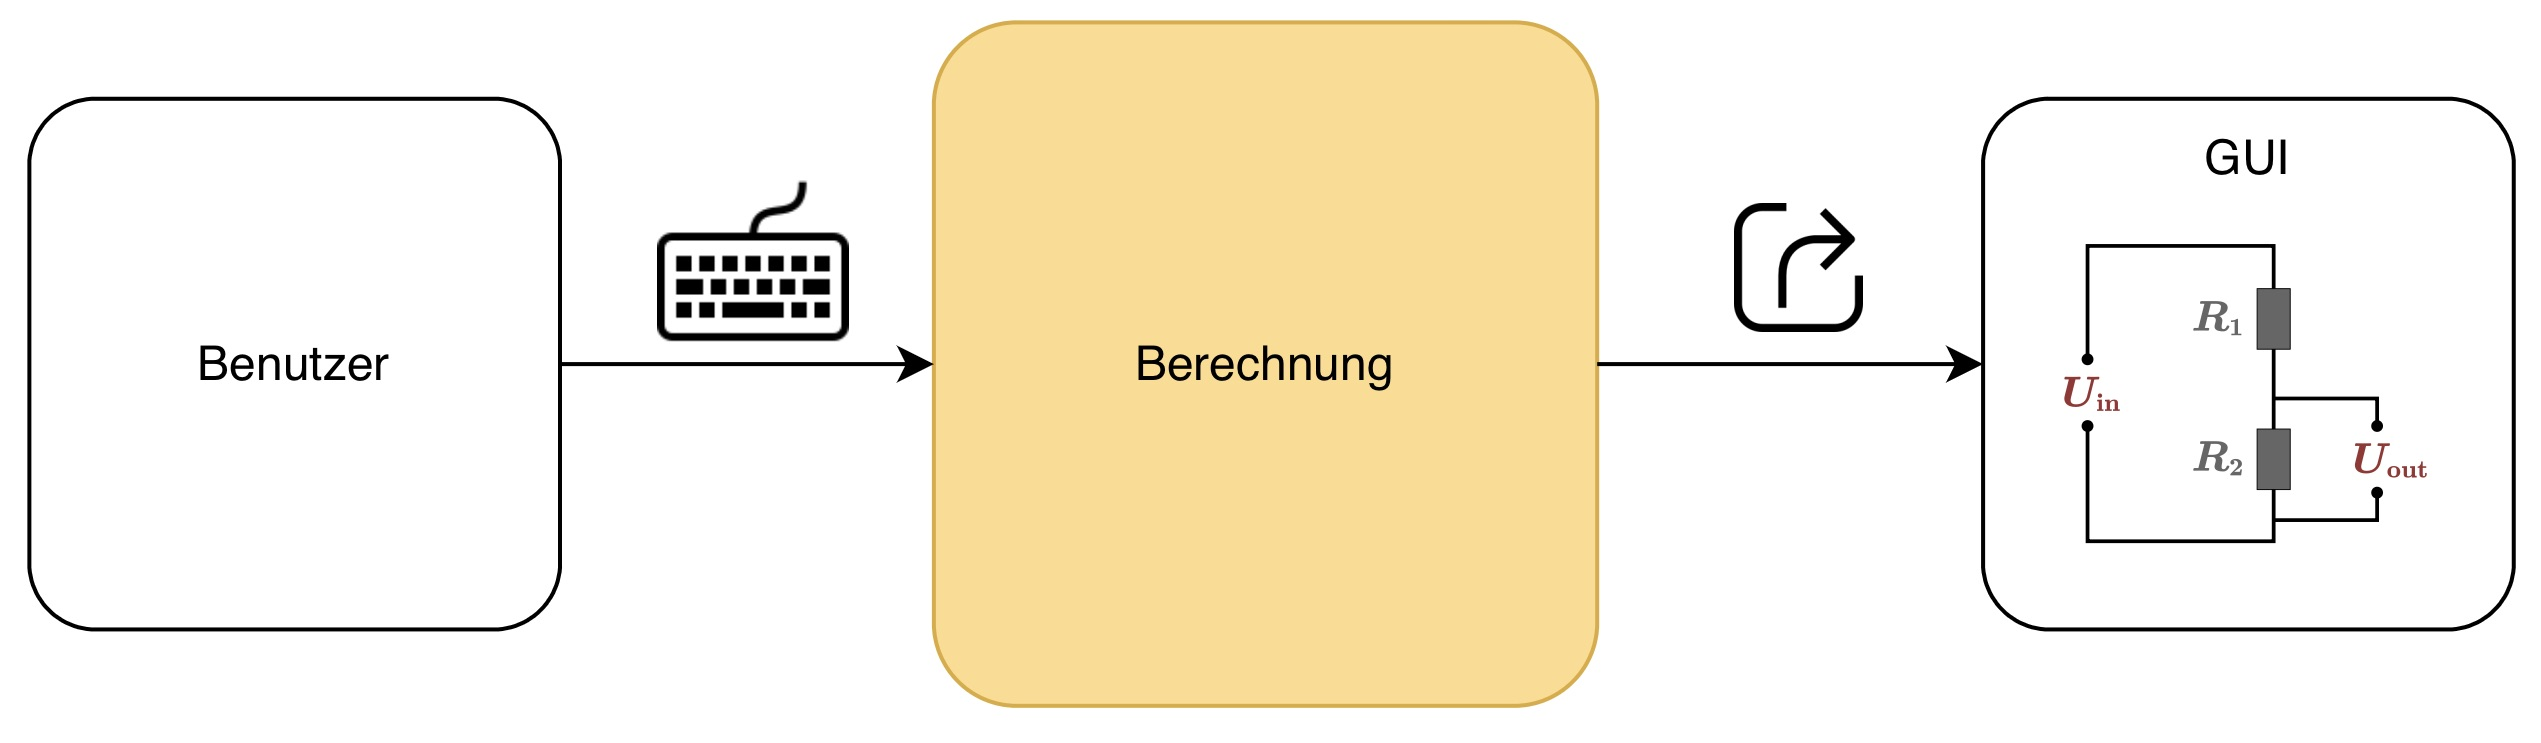
\includegraphics[width=12cm]{./images/Block.png}
	\caption{Blockschaltbild des Widerstands-Berechnungstools}
	\label{fig:blockdiagram}
\end{figure}

\subsection{Definitionen, Akronyme und Abkürzungen}
Keine
%\note{(Optional) Define all terms, acronyms, and abbreviations used in this document. This often goes into a separate document in a larger project.}

\subsection{Referenzen}
Siehe Anhang \ref{anx:ref} auf Seite \pageref{anx:ref} dieses Dokuments.
	\section{Projektstrukturplan}
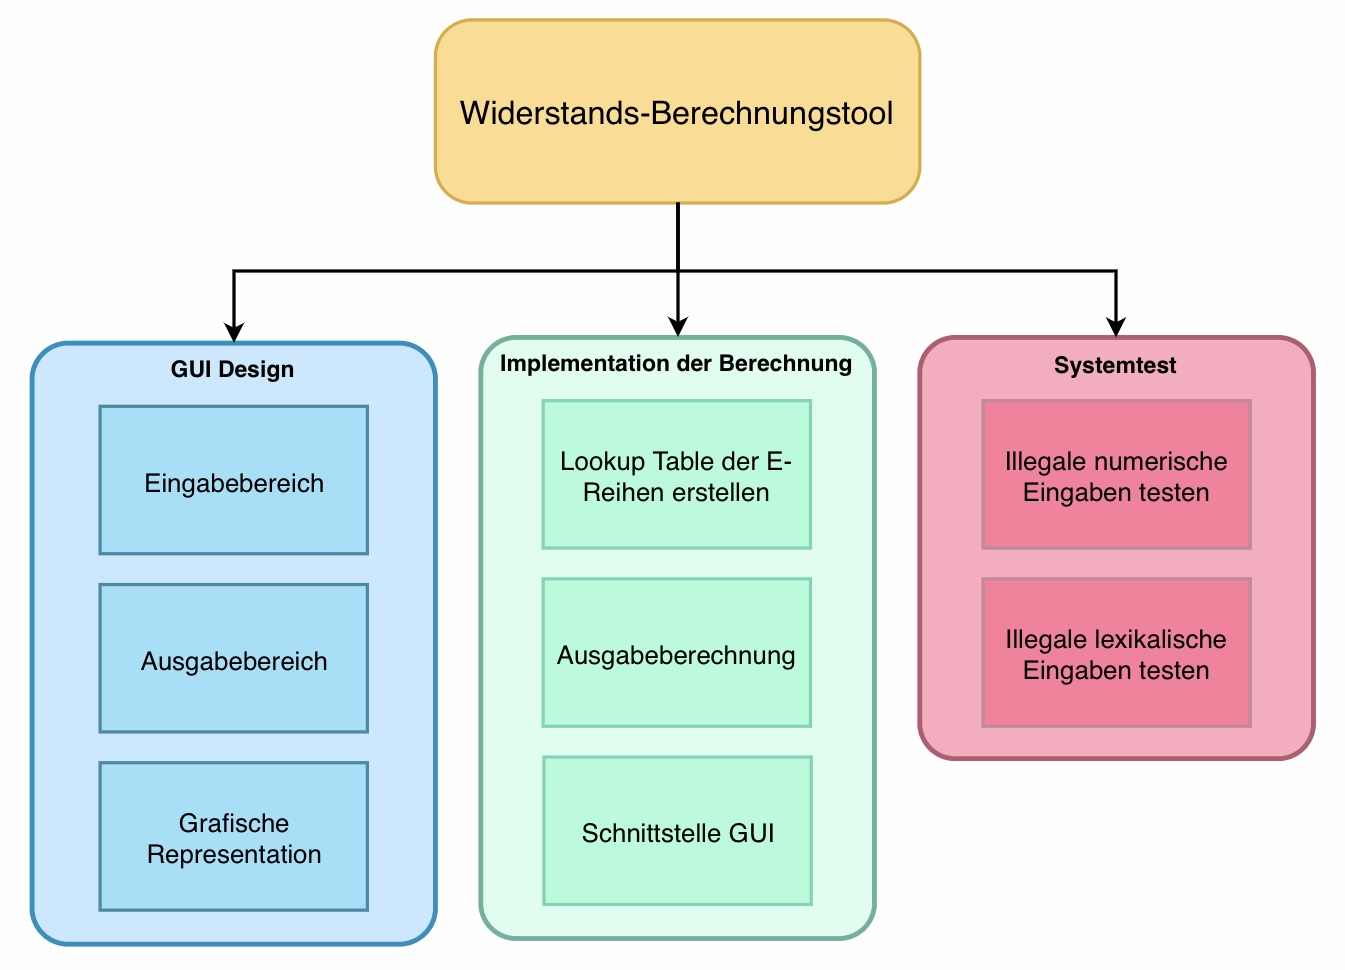
\includegraphics[width=14cm]{images/Projektstrukturplan}

\subsection{GUI-Design}
\subsubsection{Eingabebereich}
\subsubsection{Ausgabebereich}
\subsubsection{Grafische Representation}
\subsection{Implementation der Berechnung}
\subsubsection{Lookup Table der E-Reihen erstellen}
\subsubsection{Ausgabeberechnung}
\subsubsection{Schnittstelle GUI}
\subsection{Systemtest}
\subsubsection{Illegale numerische Eingaben testen}
\subsubsection{Illegale lexikalische Eingaben testen}

	\begin{landscape}
	\section{Terminplan}
	\centering
	\begin{table}[h!]
		\begin{tabular}{|l|c|c|c|c|c|c|c|c|c|}
			 \Xhline{1pt}
			 \textbf{Arbeitspaket} & \textbf{SW6} & \textbf{SW7} & \textbf{SW8} & \textbf{SW9} & \textbf{SW10} & \textbf{SW11} & \textbf{SW12} & \textbf{SW13} & \textbf{SW14} \\
			 \Xhline{0.5pt} \hline \hline
			 \textbf{GUI-Design}&&&&&&&&&\\\hline
			 
			 \multirow{2}{*}{Grafische Representation} &&& \cellcolor{red}4h &&& \cellcolor{grey} & \cellcolor{grey} & \cellcolor{grey} & \cellcolor{grey} \\\cline{2-10}
			  &&&&&&&&&\\\hline
			 
			 \multirow{2}{*}{Eingabebereich} &&& \cellcolor{red}3h &&& \cellcolor{grey} & \cellcolor{grey} & \cellcolor{grey} & \cellcolor{grey}\\\cline{2-10}
			 &&&&&&&&&\\\hline
			 
			 \multirow{2}{*}{Ausgabebereich} &&& \cellcolor{red}3h &&& \cellcolor{grey} & \cellcolor{grey} & \cellcolor{grey} & \cellcolor{grey}\\\cline{2-10}
			 &&&&&&&&&\\\hline \hline
			 
			 \textbf{Implementation Berechnung} &&&&&&&&& \\\hline
			 \multirow{2}{*}{Lookup Table der E-Reihe erstellen} &&&& \cellcolor{green}1h &&\cellcolor{grey} & \cellcolor{grey} & \cellcolor{grey} & \cellcolor{grey}\\\cline{2-10}
			 &&&&&&&&&\\\hline
			 
			 \multirow{2}{*}{Ausgabeberechnung} &&&& \cellcolor{green}3h &&\cellcolor{grey} & \cellcolor{grey} & \cellcolor{grey} & \cellcolor{grey}\\\cline{2-10}
			 &&&&&&&&&\\\hline
			 
			 \multirow{2}{*}{Schnittstelle GUI} &&&& \cellcolor{green} 4h &&\cellcolor{grey} & \cellcolor{grey} & \cellcolor{grey} & \cellcolor{grey}\\ \cline{2-10}
			 &&&&&&&&&\\\hline \hline
			 
			 \textbf{Systemtest} &&&&&&&&& \\\hline
			 \multirow{2}{*}{Illegale numerische Eingaben implementieren/testen}&&&&& \cellcolor{blue}8h & \cellcolor{grey} & \cellcolor{grey} & \cellcolor{grey} & \cellcolor{grey}\\\cline{2-10}
			 &&&&&&&&&\\\hline
			 
			  \multirow{2}{*}{Illegale lexikalische Eingaben implementieren/testen}&&&&& \cellcolor{yellow}8h & \cellcolor{grey} & \cellcolor{grey} & \cellcolor{grey} & \cellcolor{grey}\\\cline{2-10}
			 &&&&&&&&&\\\hline \hline
		 
			 \textbf{Projektabgabe} &&&&&&&&&\cellcolor{violet}  \\			 
			 \Xhline{1pt}
		\end{tabular}
	\caption{Terminplan}
	\label{table:1}
	\end{table}
	
	\begin{table}[h!]
		\centering
		\begin{minipage}{7cm}
			\begin{tabular}{|l|c|c|}
				\Xhline{1pt}
				\textbf{Bedeutung} & \textbf{Farbe Ist} & \textbf{Farbe Soll}\\
				\Xhline{0.5pt}  \hline \hline
				Flurin Arquint & \cellcolor{green} & \cellcolor{greenLight}\\ \hline
				Fabian Söllner & \cellcolor{blue} & \cellcolor{blueLight}\\ \hline
				Simeon Roth & \cellcolor{red} & \cellcolor{redLight}\\ \hline
				\Xhline{1pt}
			\end{tabular}
		\end{minipage}
	%
	\begin{minipage}{0.5cm}
		\-\
	\end{minipage}
%
\begin{minipage}{7cm}
	\begin{tabular}{|l|c|c|}
	\Xhline{1pt}
	\textbf{Bedeutung} & \textbf{Farbe Ist} & \textbf{Farbe Soll}\\
	\Xhline{0.5pt}  \hline \hline
	Christoph Hälg & \cellcolor{yellow} & \cellcolor{yellowLight}\\ \hline
	Timebuffer & \cellcolor{grey} & \cellcolor{grey}\\	 
	\Xhline{1pt}
\end{tabular}

\end{minipage}
		\caption{Legende}
		\label{table:1}
	

	\end{table}
\end{landscape} 


	\section{Funktionale Anforderungen}
\label{sec:funcReqs}
%\note{Die funktionalen Anforderungen sind die wichtigsten Teile zur Beschreibung des Systems. Für die Beschreibung der funktionalen Anforderungen bieten sich Use Cases an, nicht nur für Software, sondern auch für das ganze System. Jeder Use Case beschreibt dabei eine Funktion. Im folgenden Raster ist vorgesehen, dass bei jedem Use Case auch nicht funktionale Anforderungen wie Antwortzeiten, etc. direkt beim Use Case stehen, falls diese zu dieser Funktion gehören.

%Bei der Use Case Definition ist wichtig, dass die Granularität nicht zu fein gewählt wird. Allfällige Ausnahmefälle einer Funktion sollen beispielsweise in der Beschreibung des entsprechenden Use Cases geschehen und nicht allenfalls in einem "Unter-Use Case". 

%Statt mittels Use Cases kann dieses Kapitel auch mit \textbf{Systemfunktion 1}, \textbf{Systemfunktion 2}, etc. gegliedert werden.}


\subsection{Überblick über die Systemfunktionen}
Die folgenden Use Cases beziehen sich auf die Abbildung \ref{fig:contextDiagram} auf der Seite \pageref{fig:contextDiagram}.
%\note{Hier kommt ein Use Case Diagramm hinein, das alle Funktionen zeigt. Allenfalls genügt ein Link zum Abschnitt Systemübersicht.}


\subsection{Actors}
%\note{Kurzbeschreibung der Actors.}
\begin{tabular}{|l|l|}
	\hline
	\textbf{Actor} & \textbf{Beschreibung}\\
	\hline
	User & Gibt Eingabeparameter ein. (z.B. Ausgangsspannung)\\
	\hline
	GUI & Grafische Oberfläche zur Darstellung der Ein- und Ausgabewerte.\\
	\hline
	
\end{tabular}

\subsection{Kurzbeschreibung der Use Cases}
%\note{Jeder einzelne Use Case soll kurz beschrieben werden.}
\begin{tabular}{|l|p{13cm}|}
	\hline
	\textbf{Use Case} & \textbf{Beschreibung}\\
	\hline
	Parameter eingeben & Der User setzt die gewünschte E-Reihe sowie Ein- und Ausgangsspannung.\\
	\hline
	Ausgabe berechnen & Entsprechend der Eingabeparameter werden die beiden passendsten Widerstände ermittelt\\
	\hline
\end{tabular}
\newpage

\subsection{Use Case [Parameter eingeben]}
%\note{Ist für jeden Use Case zu beschreiben. Die folgenden Unterkapitel sollen für jeden einzelnen Use Case vollständig vorhanden sein. Falls bei einem Abschnitt nichts zu schreiben ist, dann soll dies entsprechend vermerkt werden, z.B. falls ein Use Case keine Vorbedingungen braucht oder keine nicht-funktionalen Anforderungen vorhanden sind, kann bei diesem Abschnitt einfach das Wort "keine" stehen.}

\subsubsection{Vorbedingungen}
%\note{Zustand des Systems bevor der Use Case eintritt, z.B. kann hier stehen, dass ein System erfolgreich initialisiert sein muss, damit diese Funktion ausgeführt werden kann.}
Keine

\subsubsection{Nachbedingungen}
%\note{Zustand des Systems nachdem der Use Case durchlaufen ist, z.B. kann hier bei einem Kalibrations-Use Case stehen, dass das System kalibriert oder allenfalls in einem Fehlerzustand ist.}
Keine

\subsubsection{Nicht-funktionale Anforderungen}
%\note{Zusicherungen, die für Design und Realisierung wichtig sind, wie z.B. Antwortzeit, Häufigkeit, Priorität usw.}
Keine

\subsubsection{Hauptszenario}
%\note{Beschreibung des Use Cases, ggf. gegliedert in Einzelpunkte. Beschrieben wird der Normalfall. Variationen werden mit Unterszenario-Nummer erwähnt (\textit{\textbf{[S-1]}} , \textit{\textbf{[S-2]}}, usw.) und separat als Unterszenarien beschrieben. Fehlerfälle werden mit Fehlerszenario-Nummern angegeben (\textit{\textbf{[E-1]}}, \textit{\textbf{[E-2]}}, usw.) und separat als Fehlerszenarien beschrieben.

%
%Beispiele:
%Falls gewünscht können zusätzliche Informationen erfasst werden \textit{\textbf{[S-1]}}.
%
%Beim Einlesen der Daten können die Fehler \textit{\textbf{[E-1]}}, \textit{\textbf{[E-2]}} oder \textit{\textbf{[E-3]}} auftreten.}}

%\subsubsection{Unterszenarien}
%\note{\textit{\textbf{[S-1]}} Zusatzinformationen erfassen
%
%\textit{\textbf{[S-2]}} ...}
%
%\paragraph{\textit{\textbf{[S-1]}} Zusatzinformationen erfassen}
%\paragraph{\textit{\textbf{[S-2]}} ...}
Der User gibt die gewünschte E-Reihe sowie Ein- und Ausgangsspannung ins GUI ein.


\subsubsection{Fehlerszenarien}
%\note{\textit{\textbf{[E-1]}} 
%\textit{\textbf{[E-2]}} Falsches Datenformat
%\textit{\textbf{[E-3]}} ...}

\paragraph{\textit{\textbf{[E-1]}} Eingabe von negativen Spannungswerten oder nicht numerischen Zeichen.}
%\paragraph{\textit{\textbf{[E-1]}} Falsches Datenformat}
%\paragraph{\textit{\textbf{[E-2]}} ...}

\subsubsection{Regeln}
%\note{Gültigkeits- und Validierungsregeln, Berechnungsformeln usw.}
Es dürfen nur positive Spannungen eingegeben werden.

\subsubsection{Anmerkungen}
Keine

\subsubsection{Beispiele}
Keine
\newpage

\subsection{Use Case [Ausgabe berechnen]}
%\note{Ist für jeden Use Case zu beschreiben. Die folgenden Unterkapitel sollen für jeden einzelnen Use Case vollständig vorhanden sein. Falls bei einem Abschnitt nichts zu schreiben ist, dann soll dies entsprechend vermerkt werden, z.B. falls ein Use Case keine Vorbedingungen braucht oder keine nicht-funktionalen Anforderungen vorhanden sind, kann bei diesem Abschnitt einfach das Wort "keine" stehen.}

\subsubsection{Vorbedingungen}
%\note{Zustand des Systems bevor der Use Case eintritt, z.B. kann hier stehen, dass ein System erfolgreich initialisiert sein muss, damit diese Funktion ausgeführt werden kann.}
Es wurde eine gültige Eingabe getätigt.

\subsubsection{Nachbedingungen}
%\note{Zustand des Systems nachdem der Use Case durchlaufen ist, z.B. kann hier bei einem Kalibrations-Use Case stehen, dass das System kalibriert oder allenfalls in einem Fehlerzustand ist.}
Keine

\subsubsection{Nicht-funktionale Anforderungen}
%\note{Zusicherungen, die für Design und Realisierung wichtig sind, wie z.B. Antwortzeit, Häufigkeit, Priorität usw.}
Keine

\subsubsection{Hauptszenario}
%\note{Beschreibung des Use Cases, ggf. gegliedert in Einzelpunkte. Beschrieben wird der Normalfall. Variationen werden mit Unterszenario-Nummer erwähnt (\textit{\textbf{[S-1]}} , \textit{\textbf{[S-2]}}, usw.) und separat als Unterszenarien beschrieben. Fehlerfälle werden mit Fehlerszenario-Nummern angegeben (\textit{\textbf{[E-1]}}, \textit{\textbf{[E-2]}}, usw.) und separat als Fehlerszenarien beschrieben.
Die Widerstandswerte werden berechnet und die passendsten Widerstände aus der gewählten E-Reihe ermittelt und ausgegeben.
%
%Beispiele:
%Falls gewünscht können zusätzliche Informationen erfasst werden \textit{\textbf{[S-1]}}.
%
%Beim Einlesen der Daten können die Fehler \textit{\textbf{[E-1]}}, \textit{\textbf{[E-2]}} oder \textit{\textbf{[E-3]}} auftreten.}}

%\subsubsection{Unterszenarien}
%\note{\textit{\textbf{[S-1]}} Zusatzinformationen erfassen
%
%\textit{\textbf{[S-2]}} ...}
%
%\paragraph{\textit{\textbf{[S-1]}} Zusatzinformationen erfassen}
%\paragraph{\textit{\textbf{[S-2]}} ...}



\subsubsection{Fehlerszenarien}
%\note{\textit{\textbf{[E-1]}} 
%\textit{\textbf{[E-2]}} Falsches Datenformat
%\textit{\textbf{[E-3]}} ...}

%\paragraph{\textit{\textbf{[E-1]}}Inhalt}
%\paragraph{\textit{\textbf{[E-1]}} Falsches Datenformat}
%\paragraph{\textit{\textbf{[E-2]}} ...}

\subsubsection{Regeln}
%\note{Gültigkeits- und Validierungsregeln, Berechnungsformeln usw.}
Mithilfe der Spannungsteiler-Formel werden die Widerstände R1, R2 berechnet.\\
Spannungsteiler-Formel: $U_a = U_e\cdot \dfrac{R2}{R1+R2}$

\subsubsection{Anmerkungen}
Keine

\subsubsection{Beispiele}
Keine
	
\end{document}